% THIS IS SIGPROC-SP.TEX - VERSION 3.1
% WORKS WITH V3.2SP OF ACM_PROC_ARTICLE-SP.CLS
% APRIL 2009
%
% It is an example file showing how to use the 'acm_proc_article-sp.cls' V3.2SP
% LaTeX2e document class file for Conference Proceedings submissions.
% ----------------------------------------------------------------------------------------------------------------
% This .tex file (and associated .cls V3.2SP) *DOES NOT* produce:
%       1) The Permission Statement
%       2) The Conference (location) Info information
%       3) The Copyright Line with ACM data
%       4) Page numbering
% ---------------------------------------------------------------------------------------------------------------
% It is an example which *does* use the .bib file (from which the .bbl file
% is produced).
% REMEMBER HOWEVER: After having produced the .bbl file,
% and prior to final submission,
% you need to 'insert'  your .bbl file into your source .tex file so as to provide
% ONE 'self-contained' source file.
%
% Questions regarding SIGS should be sent to
% Adrienne Griscti ---> griscti@acm.orghttps://www.overleaf.com/7267312825nsgbbwvhhrxchttps://www.overleaf.com/7267312825nsgbbwvhhrxc
%
% Questions/suggestions regarding the guidelines, .tex and .cls files, etc. to
% Gerald Murray ---> murray@hq.acm.org
%
% For tracking purposes - this is V3.1SP - APRIL 2009

\documentclass{edm_template}

\usepackage{tikz}
\usetikzlibrary{bayesnet}
\usetikzlibrary{arrows}
\usepackage{enumitem}
\usepackage{amsmath}

% \usepackage[dvipsnames]{xcolor}

\providecommand{\am}[1]{{\color{blue} [AM: #1]}}
\providecommand{\ng}[1]{{\color{red} [NG: #1]}}

\begin{document}

\title{Latent Variable Models of Enrollment for Course Planning and Understanding}

\numberofauthors{5} %  in this sample file, there are a *total*
% of EIGHT authors. SIX appear on the 'first-page' (for formatting
% reasons) and the remaining two appear in the \additionalauthors section.
%
\author{
% You can go ahead and credit any number of authors here,
% e.g. one 'row of three' or two rows (consisting of one row of three
% and a second row of one, two or three).
%
% The command \alignauthor (no curly braces needed) should
% precede each author name, affiliation/snail-mail address and
% e-mail address. Additionally, tag each line of
% affiliation/address with \affaddr, and tag the
% e-mail address with \email.
%
\alignauthor Nate Gruver \\
       \affaddr{Stanford University}\\
       \email{ngruver@cs.stanford.edu}
\alignauthor Ali Malik \\
       \affaddr{Stanford University}\\
       \email{malikali@cs.stanford.edu}
\alignauthor Brahm Capoor \\
       \affaddr{Stanford University}\\
       \email{brahm@cs.stanford.edu}
\and
\alignauthor Chris Piech\\
       \affaddr{Stanford University}\\
       \email{piech@cs.stanford.edu}
\alignauthor Andreas Paepcke \\
       \affaddr{Stanford University}\\
       \email{paepcke@cs.stanford.edu}
}
% There's nothing stopping you putting the seventh, eighth, etc.
% author on the opening page (as the 'third row') but we ask,
% for aesthetic reasons that you place these 'additional authors'
% in the \additional authors block, viz.

% Just remember to make sure that the TOTAL number of authors
% is the number that will appear on the first page PLUS the
% number that will appear in the \additionalauthors section.

\maketitle
\begin{abstract}
Administrators and students in post-secondary institutions often make impactful decisions without good quantitative models of student enrollment. Such models would give students more perspective about the space of possible course trajectories and allow administrators to simulate the effects of structural changes. We propose a generative model of course enrollment in the form of a time-dependent hidden Markov model. This model uses a real-valued relaxation of binary course enrollments to tractably model the joint probability over all possible courses. The resulting latent variable model with Gaussian emission probabilities is trained by gradient descent on a log-likelihood objective, and validation is performed by comparison with null models and the distance between sample distributions and hold-outs. Finally, three uses cases for the model are demonstrated using historical enrollments. 
\end{abstract}

%% A category with the (minimum) three required fields
%\category{H.4}{Information Systems Applications}{Miscellaneous}
%%A category including the fourth, optional field follows...
%\category{D.2.8}{Software Engineering}{Metrics}[complexity measures, performance measures]
%
%\terms{Theory}

\keywords{Enrollment modeling, mixture models, hidden Markov model} % NOT required for Proceedings

\section{Introduction}

Understanding the enrollment decisions of students in post-secondary institutions is central to the success of university administrators, researchers, and advisors. Despite this, students and staff rely primarily on heuristically constructed lists and complex mental models shared collectively through word-of-mouth for the bulk of course planning. Although work has been devoted to predicting course enrollments, few studies have come close to replicating the robust framework experienced students hold within their head---one that is capable of imagining counterfactual paths, inferring intentions, or detecting anomalies in various course planning scenarios.

To handle these more nuanced tasks, we propose a generative model of course enrollment. The distinguishing feature of a generative model is its ability to model the full joint distribution over all variables in question, in our case a student's boolean enrollments. This increased expressiveness makes it possible to calculate any desired conditional or marginal probability (though there is no guarantee of tractability in general). Arguably most of the tasks above can be described in probabilistic language. An anomalous set of enrollments, for instance, is simply one that has very low probability under a plausible model.

In this work we focus on three motivating use cases for such a model:
\begin{enumerate}[noitemsep,topsep=0pt]
	\item A student prototyping their set of future enrollments based on common paths, i.e. queries of the form
	$$\text{P}(\text{Course}_i \mid \text{Course}_{j \neq i})$$ 
	\item An advisor wondering if their advisee is on track, i.e. queries of the form
	$$P(\text{Student's enrollments} \mid \text{All other student enrollments})$$
	\item An administrator wondering about optimal resource allocation, i.e. queries of the form
	$$P(\text{All future enrollments} \mid \text{All past enrollments})$$
\end{enumerate}

\subsection{Prior Work}

Much of the prior work on enrollment modeling in the university setting is dedicated purely to predictive models, both of future course enrollment \cite{kardan2013prediction}\cite{nandeshwar2009enrollment}\cite{song1993new} and academic performance \cite{kovacic2010early}\cite{hlosta2017ouroboros}. The rise of MOOCs has also been accompanied by a flurry of work predicting and tracking online student success and engagement through course decisions \cite{balakrishnan2013predicting}\cite{Gardner2018StudentSP}\cite{AlShabandar2018TheAO}. The techniques used in these predictive tasks range from simple probabilistic models to deep neural networks. A related body of work is that on recommender systems for course enrollment, with similar neural network~\cite{Jiang2018GoalbasedCR} and probabilistic approaches~\cite{Khorasani2016AMC}. 

Another significant branch of enrollment modeling research is unsupervised learning for clustering, classification, and feature learning. Some authors focus on clustering courses with topic modeling and embedding techniques~\cite{Motz2018FindingTI}~\cite{Pardos2018AMO} while others focus instead on students--using patterns of enrollments to extract meaningful types via vector quanitization and graph analysis~\cite{Zeidenberg2011TheCO}~\cite{Slim2016TheIO}. Some even treat coenrollments as a network and extract graph-theoretic properties for representation learning~\cite{gardner2018coenrollment}~\cite{Wang2017AnalyzingCC}. 

The primary limitations found in the prior work is a lack of flexibility. Strong predictive models can be trained, but they are most discriminative instead of generative and thus lack the ability to answer nuanced inference queries about enrollment decisions conditioned on both past and future enrollments. While some approaches do achieve this level of expressiveness~\cite{Jiang2018GoalbasedCR}, they lack the ability to simulate out different high-probability sequences of enrollments--a functionality that allows students to more thoroughly prototype. 

Similarly the unsupervised approaches while often effective often don't allow for estimation of key probabilistic metrics like the posterior class probability or log likelihood of a sample. Adapting the more general probabilistic approach presented here opens the door for a much more diverse set of analyses within a shared statistical framework.

\section{Background \& Models}

There is a rich history of probabilistic modeling of categorical data in the natural language processing literature. Here we use these techniques to model enrollments as analogues of natural language tokens, with each student comprising either a set or sequence of sets of enrollments. Of particular relevance are mixture and hidden Markov models which can be used to capture the typography of students and the sequential nature of their enrollments. 

\subsection{Mixture Models}

Among the simplest and most common mixture models used in generative modeling of categorical variables with strong correlation is Latent Dirichlet allocation (LDA). In this mixture model, the hidden variable, or topic, is drawn from a multinomial distribution and then words are sampled conditioned on the topic:
\begin{align*}
\theta &\sim \text{Dir}(\alpha) \\
\text{ topic } z_i &\sim \text{Multinomial}(\theta) \\
\text{ word } w \mid z_i &\sim \text{Multinomial}(\beta) \\ 	
\end{align*}

\vspace{-7mm}
One obvious drawback of this model if that it assumes words are drawn independently given the selected topic. In the case of course enrollments this is problematic for at least two reasons: first because enrollment decisions often affect one another and second because effectively modeling enrollments requires modeling stochasticity in the number of classes taken by students. It is easier to capture these two facets of the data if we can model enrollments jointly.

Take $X_i$ to be set of enrollments for a student $i$ with 
$$X_{ij} = 
\begin{cases}
\,\,1 & $student $ i $ took class $ j \\
-1 & $otherwise$
\end{cases}
$$
Any probability distribution over all $X_i \in \{-1,1\}^m$ would require $2^m - 1$ parameters to specify and is thus impractical. We thus relax the discrete problem to a real-valued vector space with $\bar{X}_i \in \mathbb{R}^m$ and $X_{ij} = \text{sign}(\bar{X}_{ij})$. With this alternative encoding of enrollments we can model all enrollments jointly with a multivariate normal distribution. Though at face value this seems like an odd choice, the resulting model is akin to any Energy-Based Model that places the highest density on a particular assignment to the variables with the likelihood decreasing with distance from the modal assignment. 

With the real-valued relaxation we can define a Gaussian mixture model that relies on a latent categorical variable and a multivariate normal distribution  from which observed samples are drawn. In particular
\vspace{-7mm}

\begin{align*}
h_i &\sim \text{Multinomial}(\theta) \\
\bar{X} \mid h_i &\sim \mathcal{N}(\mu_i, \Sigma_i) \\
\end{align*}

\vspace{-7mm}
A graphical representation of a the mixture model with hidden categorical variable $h$ and observed enrollment vector $\bar{X}$ is shown in Figure \ref{fig:mixture_model}. 

\begin{figure}
	\centering
	\tikz{
	% nodes
	\node[obs] (X0) {$X_i$};%
	\node[latent,above=of X0] (h0) {$h_i$}; %
	\node[latent,rectangle,left=of h0] (theta0) {$\theta$}; %
	\node[latent,rectangle,left=of X0] (params0) {$\mu_k, \Sigma_k$}; %
	
	\node[latent,rectangle,right=1.5cm of X0] (params1) {$\mu_k, \Sigma_k$}; %
  	\node[latent,rectangle,right=1.5cm of h0] (theta1) {$\theta, \phi$}; %
	
	\node[obs,right=of params1] (X1) {$X^t_i$};%
	\node[latent,above=of X1] (h1) {$h^t_i$}; %
	
	% plate
	\plate [inner sep=.25cm,yshift=.2cm] {plate0} {(X0)(h0)} {$N$}; %
	\plate [inner sep=.25cm,yshift=.2cm] {plate1} {(X1)(h1)} {$N$}; %
	\plate [inner sep=.25cm,yshift=.2cm] {plate2} {(params0)} {$K$}; %
	\plate [inner sep=.25cm,yshift=.2cm] {plate3} {(params1)} {$K$}; %
	
	% edges
	\edge {h0} {X0}  
	\edge {theta0} {h0}
	\edge {params0} {X0}
	
	\edge {h1} {X1}
    \edge {theta1} {h1}
	\edge {params1} {X1}
	\draw (h1) edge[loop above] node {} (h1)}
	\caption{\label{fig:mixture_model} Graphical representation of mixture model (left) and hidden Markov model (right) using plate notation}
\end{figure}

\subsection{Contextual Mixture Model}

A common extension of a mixture to sequential data is the Hidden Markov Model (HMM), which formulates the latent variables as a Markov chain. Though the recursive definition of a HMM is useful in many practical applications, in the case of enrollments we can assert a stronger prior over the strictly sequential nature of hidden states (Figure~\ref{fig:contextual_mixture_model}). For a general HMM with Gaussian emission probabilities, we have 
\begin{align*}
h^0 &\sim \text{Multinomial}(\theta) \\    
h^{t+1} \mid h^{t} &\sim \text{Multinomial}(\phi) \\
x^{t} \mid h_i^{t} &\sim \mathcal{N}(\mu_i, \Sigma_i)
\end{align*}
In contrast, for a ``contextual" mixture model we have 
\begin{align*}
h^0 &\sim \text{Multinomial}(\theta) \\    
h^{t+1} \mid h^{t} &\sim \text{Multinomial}(\phi^t) \\
x^{t} \mid h_i^{t} &\sim \mathcal{N}(\mu^t_i, \Sigma^t_i)
\end{align*}
Note that the parameters of the transition and emission distributions are different for each timestep. In general any contextual mixture model can be expressed using a hidden Markov model, but enforcing the form above allows us to incorporate priors that significantly improve the chances of training a plausible model.

For any contextual mixture model over $T$ timesteps we have
\begin{align*}
ll(\mathcal{D}, \, &h^{0:T} ; \, \theta,\phi^{1:T},\mu^{1:T},\Sigma^{1:T}) \, = \\
&\sum_{i=1}^N \log P(h^0) + \sum_{t=1}^T \log P(X^t_i \mid h^t) + \log P(h^t \mid h^{t-1})
\end{align*}
Thus $ll(\mathcal{D})$, the log-likelihood of the data, can be obtained by marginalization of the hidden variables. Training of the model can be performed with Expectation-Maximization via an algorithm analogous to the Baum-Welch algorithm (parameter updates given the appendix) or via gradient descent on the negative log-likelihood. In this work we opted for gradient descent because of the available software for parallel computation offering a substantial speedup for larger datasets. 

In order to make learning of $\Sigma^t_i$ possible given the constraint of positive semi-definiteness, we parametrize the multivariate normals by $\mu_i^t$ and the Cholesky decomposition, $T$, of each precision matrix, $(\Sigma^t_i)^{-1}$, with $TT^\top = (\Sigma^t_i)^{-1}$. Samples can thus be drawn from each Gaussian via 
$$\bar{X} = \mu + T^{-\top} z$$ 
for $z$ a random vector in $\mathbb{R}^m$. 

One could rightly point out that HMM-style models have been largely phased-out by models built around Recurrent Neural Networks in state-of-the-art NLP settings and thus question why we choose a simpler generative model. Our choice was made with at least two important factors in mind. First, in the current setting in which we seek a model for understanding as much as optimal prediction of enrollments, the small discrete latent space of our model offers highly interpretable representations compared with the continuous latent vector space of neural architecture. Second, for the applications we described in the introduction, a fully generative model is necessary. Only highly complex variational neural architectures are capable of all the inference queries we describe, and we had little faith in the ability of these models to train effectively on small datasets. 

\begin{figure}
    \centering
	\tikz{
	% nodes
	\node[obs] (X0) {$X^0_i$};%
	\node[latent,above=of X0] (h0) {$h^0_i$}; %
	\node[latent,rectangle,above=of h0] (theta0) {$\theta^0$}; %
	\node[latent,rectangle,below=of X0] (params0) {$\mu^0, \Sigma^0$}; %	
	
	\node[obs,right=of X0] (X1) {$X^1_i$};%
	\node[latent,above=of X1] (h1) {$h^1_i$}; %
	\node[latent,rectangle,above=of h1] (theta1) {$\theta^1,\phi^1$}; %
	\node[latent,rectangle,below=of X1] (params1) {$\mu^1, \Sigma^1$}; %	
	
	\node[obs,right=of X1] (X2) {$X^2_i$};%
	\node[latent,above=of X2] (h2) {$h^2_i$}; %
	\node[latent,rectangle,above=of h2] (theta2) {$\theta^2,\phi^2$}; %
	\node[latent,rectangle,below=of X2] (params2) {$\mu^2, \Sigma^2$}; %	

	\node[obs,right=of X2] (X3) {$X^3_i$};%
	\node[latent,above=of X3] (h3) {$h^3_i$}; %
	\node[latent,rectangle,above=of h3] (theta3) {$\theta^3,\phi^3$}; %
	\node[latent,rectangle,below=of X3] (params3) {$\mu^3, \Sigma^3$}; %	
	
	% plate
	\plate [inner sep=.25cm,yshift=.2cm] {plate0} {(X0)(X1)(X2)(X3)(h0)(h1)(h2)(h3)} {$N$}; %
 	\plate [inner sep=.25cm,yshift=.2cm] {plate1} {(params0)(params1)(params2)(params3)} {$K$}; %
	
	% edges 
	\edge {theta0} {h0}
	\edge {h0} {X0}
	\edge {params0} {X0}
	
	\edge {theta1} {h1}
	\edge {h0} {h1}
	\edge {h1} {X1}
	\edge {params1} {X1}
	
	\edge {theta2} {h2}
	\edge {h1} {h2}
	\edge {h2} {X2}
	\edge {params2} {X2}
	
	\edge {theta3} {h3}
	\edge {h2} {h3}
	\edge {h3} {X3}
	\edge {params3} {X3}}
	
	\caption{\label{fig:contextual_mixture_model} Graphical representation of contextual mixture model using plate notation}
\end{figure}

\section{Results}

We use 18 years of course enrollment data from a private University in the United States. The data was given in the form of 2.15 million anonymized enrollment records with fields for course name and student major. Importantly, this dataset included not only the enrollment data of full-time students but also part-time and summer school students who were removed before the model was trained. 

The training data was created by aggregating student enrollments per-year and encoding them in the $-1/1$ scheme described earlier. With this data we could train a sequential model of enrollments \textit{per-degree}. This step was not strictly necessary and degree could have been modeled latently, but as most of our motivating queries are made at the level of department, this didn't feel like a sacrifice. The results presented here are from models of the 4-year undergraduate degree programs in Computer Science, Math, and Philosophy, which were most familiar to the authors. 

As most of the resulting matrices were of dimension $(n,m)$ with $m > 10^3$, we additionally performed dimensionality reduction by removing classes that were enrolled in less than 10 times by all students of a major over the entire time period. This step also acted as a form of denoising as these enrollments tended to be less correlated with the others. 

\subsection{Model Selection}

KL-divergence plots for LDA, GMM, CGMM with equal-sized latent space

KL-divergence plots for different sized latent space for CGMM

\subsection{Visualizing Hidden Variables}

plots for CS and Philosophy departments with (x,y) location from t-SNE of course embedding and color from most common student cluster 

\subsection{Quantifying Enrollment Likelihood}

Another useful application of our generative model is in quantifying enrollment likelihood. By training a model on a fraction of the enrollments and evaluating the likelihood of the held-out enrollments, we can get a sense of how unusual the hold-out enrollments are by comparison. Taking this principle to its extreme, we can train a model for each student on every other student's enrollments, allowing us to model exactly how much each particular student varies from the typical. Figure~\ref{fig:likelihistogram} shows a histogram of the log-likelihood assigned to each undergraduate student in the computer science department using this process. In Figure~\ref{fig:piecharts} we dig into the kinds of students who fall within each region of this histogram. In particular, by examining the classes these students take, we see that the model captures at least two meaningful axes of variance: first, it recognizes that it is rare for students to take a very diverse set of courses spanning many academic subjects, and, second, it captures the spectrum of ambition, from just taking what is required within one's department to enrolling in up to 30 computer science classes. 

\begin{figure}
    \centering
    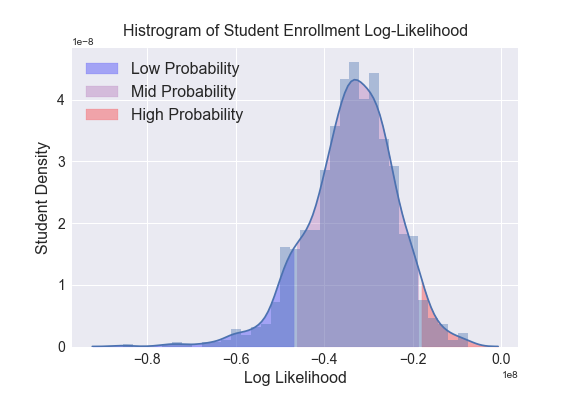
\includegraphics[scale=0.4]{figures/loglikelihood_hist.png}
    \caption{\label{fig:likelihistogram} Histogram of log-likelihoods for each student assigned by a model trained on all other students}
\end{figure}

\begin{figure}
    \centering
    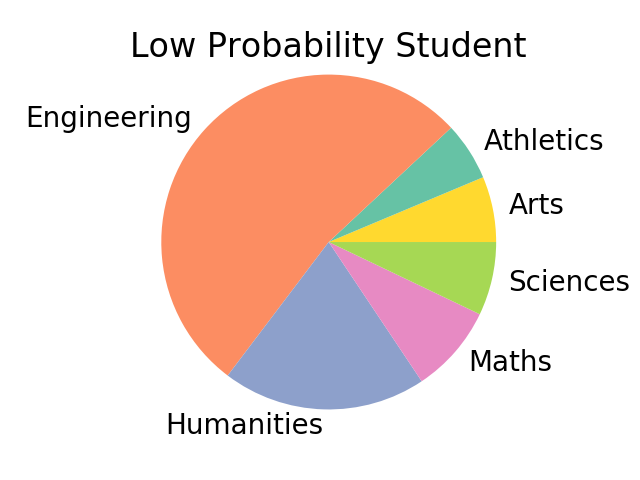
\includegraphics[scale=0.25]{figures/lowpie.png}
    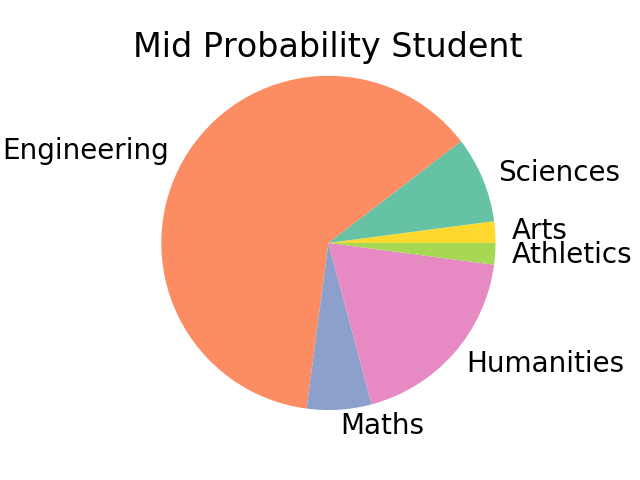
\includegraphics[scale=0.25]{figures/midpie.png} \\
    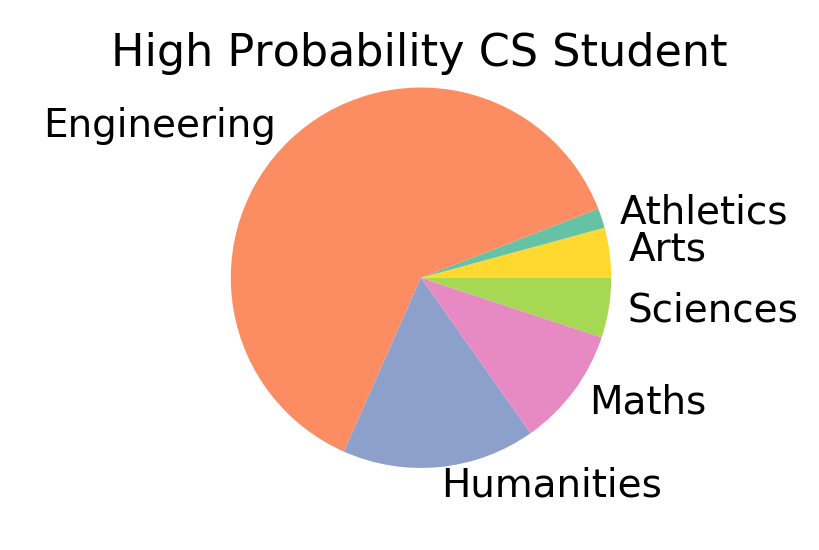
\includegraphics[scale=0.25]{figures/highpie.png}
    \caption{\label{fig:piecharts} Pie charts representing the difference between enrollment patterns captured by the model}
\end{figure}

\subsection{Sampling Paths}

Potential high-likelihood paths conditioned on given start and end point. 

\section{Discussion}


%ACKNOWLEDGMENTS are optional
\section{Acknowledgments}

%
% The following two commands are all you need in the
% initial runs of your .tex file to
% produce the bibliography for the citations in your paper.
\bibliographystyle{abbrv}
\bibliography{sigproc}  % sigproc.bib is the name of the Bibliography in this case
% You must have a proper ".bib" file
%  and remember to run:
% latex bibtex latex lvuatex
% to resolve all references
%
% ACM needs 'a single self-contained file'!
%
%APPENDICES are optional
%\balancecolumns
% \appendix
% %Appendix A
% \section{Headings in Appendices}
% The rules about hierarchical headings discussed above for
% the body of the article are different in the appendices.
% In the \textbf{appendix} environment, the command
% \textbf{section} is used to
% indicate the start of each Appendix, with alphabetic order
% designation (i.e. the first is A, the second B, etc.) and
% a title (if you include one).  So, if you need
% hierarchical structure
% \textit{within} an Appendix, start with \textbf{subsection} as the
% highest level. Here is an outline of the body of this
% document in Appendix-appropriate form:
% \subsection{Introduction}
% \subsection{The Body of the Paper}
% \subsubsection{Type Changes and  Special Characters}
% \subsubsection{Math Equations}
% \paragraph{Inline (In-text) Equations}
% \paragraph{Display Equations}
% \subsubsection{Citations}
% \subsubsection{Tables}
% \subsubsection{Figures}
% \subsubsection{Theorem-like Constructs}
% \subsubsection*{A Caveat for the \TeX\ Expert}
% \subsection{Conclusions}
% \subsection{Acknowledgments}
% \subsection{Additional Authors}
% This section is inserted by \LaTeX; you do not insert it.
% You just add the names and information in the
% \texttt{{\char'134}additionalauthors} command at the start
% of the document.
% \subsection{References}
% Generated by bibtex from your ~.bib file.  Run latex,
% then bibtex, then latex twice (to resolve references)
% to create the ~.bbl file.  Insert that ~.bbl file into
% the .tex source file and comment out
% the command \texttt{{\char'134}thebibliography}.
% % This next section command marks the start of
% % Appendix B, and does not continue the present hierarchy
% \section{More Help for the Hardy}
% The acm\_proc\_article-sp document class file itself is chock-full of succinct
% and helpful comments.  If you consider yourself a moderately
% experienced to expert user of \LaTeX, you may find reading
% it useful but please remember not to change it.
% \balancecolumns
% % That's all folks!
\end{document}
